\section{Results}

This section presents the experimental results obtained during the validation of the system. The tests are divided into unitary tests, which verify the correct operation of individual hardware components, and system-level tests, which evaluate the integrated behavior of the complete system under normal operating conditions.

\subsection{Unitary Tests}

Unitary tests were performed to validate the correct functionality of each sensor and actuator independently. These tests ensured that individual peripherals were properly configured, responsive, and capable of delivering consistent and reliable measurements before system integration.

\subsubsection{Soil Moisture}

\autoref{fig:soil_measurement_res} shows the soil moisture sensor measurements obtained during the unitary test. The sensor responds correctly to variations in moisture level, providing stable and repeatable readings that are consistent with the expected operating range.

\begin{figure}[H]
    \centering
    \includegraphics[width=0.2\textwidth]{images/soil.png}
    \caption{Soil Moisture Measurement}
    \label{fig:soil_measurement_res}
\end{figure}

\subsubsection{Phototransistor}

The phototransistor unitary test, shown in \autoref{fig:light_measurement_res}, demonstrates the system's ability to measure ambient light intensity. The measured values vary as expected with changes in illumination, confirming correct \gls{ADC} configuration and signal conditioning.

\begin{figure}[H]
    \centering
    \includegraphics[width=0.15\textwidth]{images/light.png}
    \caption{Light Measurement}
    \label{fig:light_measurement_res}
\end{figure}

\subsubsection{\acrshort{GPS}}

\autoref{fig:gps_measurement_res} presents the output of the GPS module during standalone testing. The module successfully provides geographic coordinates, altitude, satellite count, and time information, validating correct UART communication and data parsing.

\begin{figure}[H]
    \centering
    \includegraphics[width=0.99\textwidth]{images/gps.png}
    \caption{GPS Measurement}
    \label{fig:gps_measurement_res}
\end{figure}

\subsubsection{Accelerometer}

The accelerometer test results are shown in \autoref{fig:accel_measurement_res}. The sensor accurately captures acceleration values along the three spatial axes, demonstrating correct configuration of the measurement range and proper \gls{I2C} communication.

\begin{figure}[H]
    \centering
    \includegraphics[width=0.85\textwidth]{images/accel.png}
    \caption{Accelerometer Measurement}
    \label{fig:accel_measurement_res}
\end{figure}

\subsubsection{\acrshort{RGB} Colour Sensor}

Figures~\ref{fig:colors_res} and~\ref{fig:color_measurement_res} illustrate the performance of the \gls{RGB} color sensor. The sensor reliably detects variations in color intensity and provides consistent red, green, blue, and clear channel readings, enabling accurate dominant color detection.

\begin{figure}[H]
    \centering
    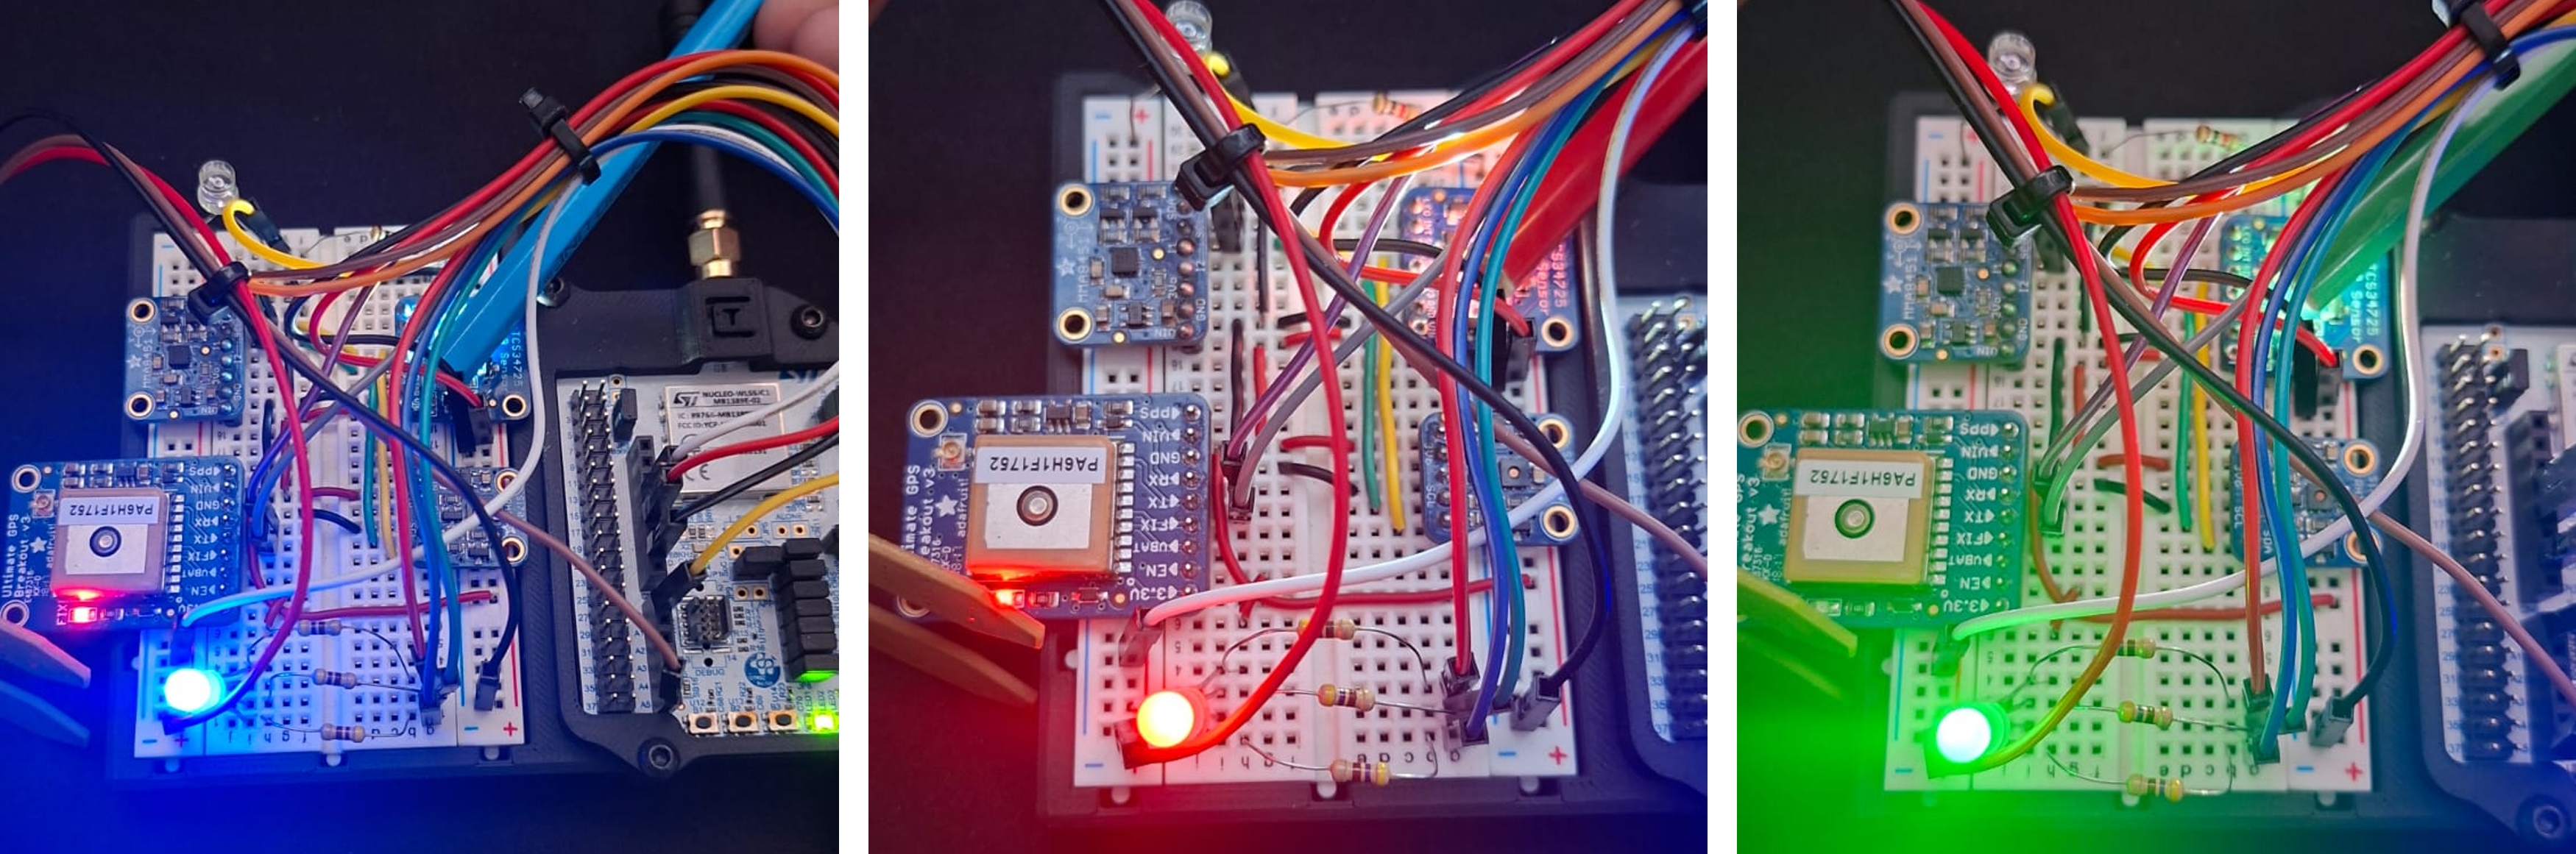
\includegraphics[width=0.8\textwidth]{images/colores.png}
    \caption{Colours}
    \label{fig:colors_res}
\end{figure}

\begin{figure}[H]
    \centering
    \includegraphics[width=0.9\textwidth]{images/color.png}
    \caption{Color Measurement}
    \label{fig:color_measurement_res}
\end{figure}

\subsubsection{Temperature and Humidity Sensor}

\autoref{fig:th_measurement_res} shows the temperature and humidity measurements obtained during testing. The sensor delivers stable and coherent values, confirming the correct resolution configuration and reliable environmental sensing.

\begin{figure}[H]
    \centering
    \includegraphics[width=0.6\textwidth]{images/th.png}
    \caption{Temperature and Humidity Measurement}
    \label{fig:th_measurement_res}
\end{figure}

\subsubsection{\acrshort{RGB} \acrshort{LED}}

The \gls{RGB} \gls{LED} unitary test, shown in \autoref{fig:rgb_led_res}, verifies the correct control of individual color channels. Each color can be independently activated, confirming proper \gls{GPIO} configuration and correct \gls{LED} driver operation.

\begin{figure}[H]
    \centering
    \includegraphics[width=0.3\textwidth]{images/rgb_led.png}
    \caption{\acrshort{RGB} \acrshort{LED}}
    \label{fig:rgb_led_res}
\end{figure}

\subsubsection{Board \acrshort{LED}s}

\autoref{fig:board_led_res} demonstrates the correct operation of the on-board \glspl{LED}. These indicators are used to provide visual feedback regarding system state and operating mode, and their correct behavior confirms proper \gls{GPIO} handling.

\begin{figure}[H]
    \centering
    \includegraphics[width=0.4\textwidth]{images/board_led.png}
    \caption{Board \acrshort{LED}s}
    \label{fig:board_led_res}
\end{figure}


\subsubsection{User button}

The user button test, shown in \autoref{fig:user_button_res}, validates correct detection of button presses and reliable interrupt handling. The button is used as the primary user interface element for changing system operating modes.

\begin{figure}[H]
    \centering
    \includegraphics[width=0.15\textwidth]{images/button.png}
    \caption{User Button}
    \label{fig:user_button_res}
\end{figure}


\subsection{System Tests}

System-level tests were conducted to evaluate the integrated behavior of all system components working together. These tests verify correct initialization, synchronized data acquisition, mode transitions, and alarm signaling.

\subsubsection{Initialization}

\autoref{fig:init_res} shows the system output during the initialization phase. All peripherals are correctly initialized, and the system reports its startup state, confirming that the hardware and software components are properly configured before entering normal operation.

\begin{figure}[H]
    \centering
    \includegraphics[width=0.75\textwidth]{images/init.png}
    \caption{Initialization}
    \label{fig:init_res}
\end{figure}

\subsubsection{Measurements}

The measurements test, illustrated in \autoref{fig:measure_res}, demonstrates the system's ability to acquire, process, and display data from all sensors simultaneously. The results confirm synchronized operation of sensor and GPS threads.

\begin{figure}[H]
    \centering
    \includegraphics[width=0.75\textwidth]{images/measurements.png}
    \caption{Measurements}
    \label{fig:measure_res}
\end{figure}


\subsubsection{Mode Changes}

\autoref{fig:modes_res} presents the system behavior during mode transitions. Each button press correctly advances the system to the next operating mode, and the corresponding visual and textual feedback confirms proper state management.

\begin{figure}[H]
    \centering
    \includegraphics[width=0.7\textwidth]{images/modes.png}
    \caption{Mode Changes}
    \label{fig:modes_res}
\end{figure}


\subsubsection{\acrshort{RGB} Dominant color (TEST MODE)}

\autoref{fig:dom_color_res} illustrates dominant color detection in Test Mode. The \gls{RGB} \gls{LED} accurately reflects the color channel with the highest intensity, validating both color sensor measurements and the dominant color selection logic.

\begin{figure}[H]
    \centering
    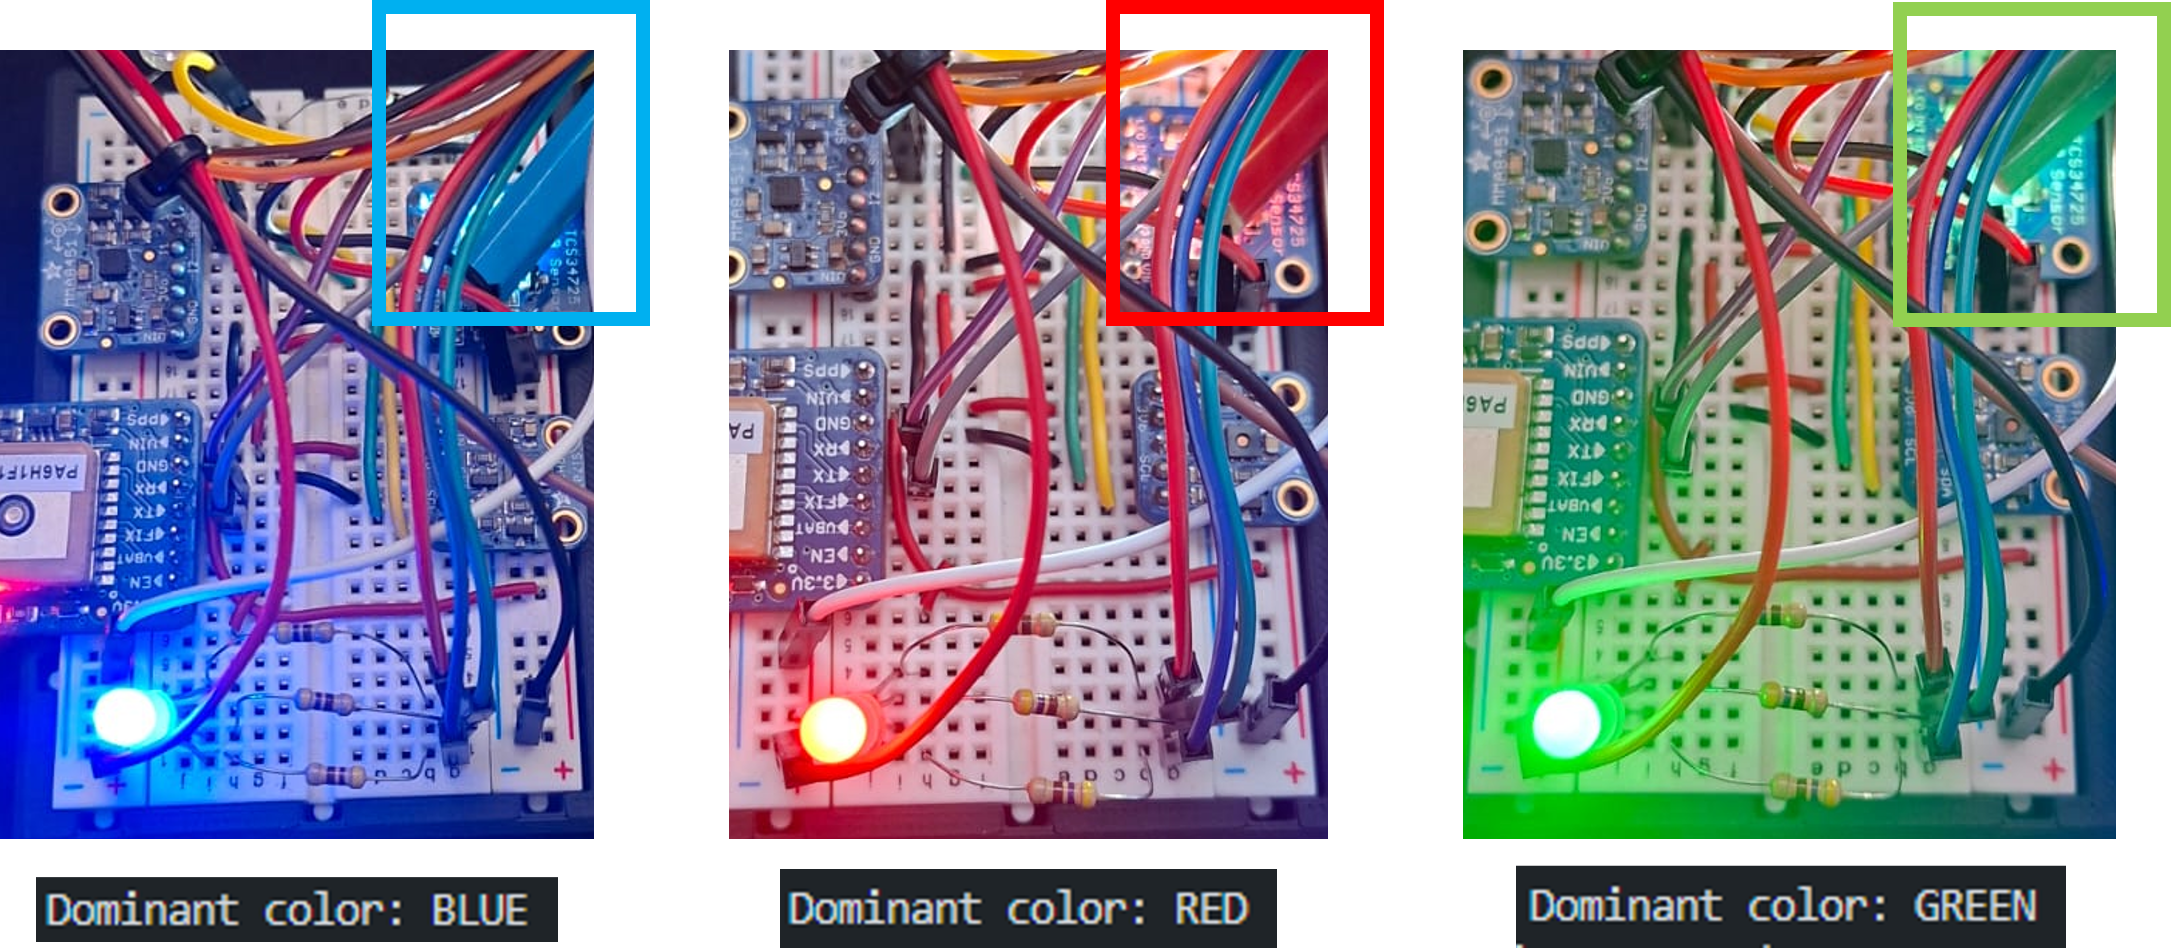
\includegraphics[width=0.99\textwidth]{images/dom_color.png}
    \caption{\acrshort{RGB} Dominant Color (TEST MODE)}
    \label{fig:dom_color_res}
\end{figure}


\subsubsection{Limits and \acrshort{RGB} Alarms (NORMAL MODE)}

In Normal Mode, sensor measurements are continuously validated against predefined limits. When a measurement exceeds its allowed range, the corresponding alarm is activated and displayed through the \gls{RGB} \gls{LED}. Multiple simultaneous alarms are handled by cyclic color indication, ensuring clear and intuitive visual feedback to the user.

For this example, the maximum temperature is set to 10C, while the minimum soil moisture is set to 10\%. As shown in \autoref{fig:alarms_res}, the alarms are triggered when the values exceed these limits. In this case, the temperature is below than 10C (red alarm) and the relative humidity is higher than 75\% (blue alarm). Later (second 16), when the soil moisture drops below 10\%, the cyan alarm is also activated. These values are clipped to the nearest limit.

\href{https://upm365-my.sharepoint.com/:v:/g/personal/estela_mora_barba_upm_es/IQAcrwEj6volTIWrmzzSXfVRAXxYS2n1ZRkFSphvheN9NaU?e=jgf2FQ&nav=eyJyZWZlcnJhbEluZm8iOnsicmVmZXJyYWxBcHAiOiJTdHJlYW1XZWJBcHAiLCJyZWZlcnJhbFZpZXciOiJTaGFyZURpYWxvZy1MaW5rIiwicmVmZXJyYWxBcHBQbGF0Zm9ybSI6IldlYiIsInJlZmVycmFsTW9kZSI6InZpZXcifX0%3D}{Video demonstration (click here)}

\begin{figure}[H]
    \centering
    \includegraphics[width=0.9\textwidth]{images/rgb_alarm.png}
    \caption{Limits and \acrshort{RGB} Alarms (NORMAL MODE)}
    \label{fig:alarms_res}
\end{figure}

\subsubsection{Statistics Report (NORMAL MODE)}

\autoref{fig:stats_res} presents the statistical report generated during Normal Mode operation. The system computes and displays mean, minimum, and maximum values for selected measurements, providing a concise summary of environmental conditions over time.

\begin{figure}[H]
    \centering
    \includegraphics[width=0.6\textwidth]{images/stats.png}
    \caption{Measurements Statistics}
    \label{fig:stats_res}
\end{figure}


\subsubsection{ADVANCED MODE}

The results of the ADVANCED MODE are presented in \autoref{adv_results}.



\subsection{External Tests}

Both CPPcheck and Valgrind are executed through GitHub Actions as part of the continuous integration pipeline. These external tools are used to perform static and dynamic analysis in order to improve code quality and detect potential issues early in the development process. Due to the specific characteristics of the Zephyr \gls{RTOS} environment and the target architecture, certain limitations are encountered during their execution.

\subsubsection{CPPcheck}

CPPcheck is used to perform static code analysis on the C/C++ modules of the project. As shown in \autoref{fig:cppcheck}, the reported warnings are limited and expected.

\begin{figure}[H]
    \centering
    \includegraphics[width=0.99\textwidth]{images/cppcheck.png}
    \caption{CPPcheck}
    \label{fig:cppcheck}
\end{figure}

Most of the messages indicate that Zephyr-specific headers and libraries cannot be found. This is caused by the fact that the GitHub Actions environment does not provide a complete Zephyr build context, and CPPcheck is executed without access to the full toolchain and board support packages required by the operating system. 

Additionally, CPPcheck reports several unused functions. This behavior is considered acceptable, as the analyzed modules are implemented as libraries, not directly for the this specific system.

No critical errors or defects were detected during this analysis, and the reported warnings do not indicate functional issues in the codebase.



\subsubsection{Valgrind}

Valgrind was configured with the objective of performing dynamic memory analysis. However, as illustrated in \autoref{fig:valgrind}, the execution was not successful.

This limitation is primarily due to the target platform. The project is based on Zephyr \gls{RTOS} and targets an \gls{ARM} architecture, while Valgrind is designed to run on Linux-based systems and does not support direct execution on embedded \gls{ARM} targets without a compatible operating system.

Moreover, multiple attempts were made to build and execute the Zephyr application within the GitHub Actions environment. These attempts were unsuccessful due to the complexity of the Zephyr build process, which requires a specific toolchain, hardware definitions, and board-level configuration that are not easily supported or emulated in a continuous integration environment.

As a result, Valgrind could not be effectively applied to this project.

\begin{figure}[H]
    \centering
    \includegraphics[width=0.99\textwidth]{images/valgrind.png}
    \caption{Valgrind}
    \label{fig:valgrind}
\end{figure}